%%%%%%%%%%%%%%%%%%%%%%%%%%%%%%%%%%%%
% Slide options
%%%%%%%%%%%%%%%%%%%%%%%%%%%%%%%%%%%%

% Option 1: Slides with solutions

\documentclass[slidestop,compress,mathserif]{beamer}
\usepackage{booktabs}
\newcommand{\soln}[1]{\textit{#1}}
\newcommand{\solnGr}[1]{#1}

% Option 2: Handouts without solutions

%\documentclass[11pt,containsverbatim,handout]{beamer}
%\usepackage{pgfpages}
%\pgfpagesuselayout{4 on 1}[letterpaper,landscape,border shrink=5mm]
%\newcommand{\soln}[1]{ }
%\newcommand{\solnGr}{ }

%%%%%%%%%%%%%%%%%%%%%%%%%%%%%%%%%%%%
% Style
%%%%%%%%%%%%%%%%%%%%%%%%%%%%%%%%%%%%
%%%%%%%%%%%%%%%%%%%%%%%%%%%%%%%%%%%%%%%%%%%%%%%%%%%%%%%%%%%%%%%%%%%%%%%%
% MA213/214 shared slide style
%
% "Calm & Cool" palette + content-type callout boxes.
% Overhauled (2026) from the original OpenIntro/metropolis style:
%   - all OpenIntro visual branding removed (logo, grid, colors)
%   - a low-key cool palette (see colors below)
%   - tcolorbox callout boxes so students recognize content types
% See common/README.md for the command cheat-sheet.
%%%%%%%%%%%%%%%%%%%%%%%%%%%%%%%%%%%%%%%%%%%%%%%%%%%%%%%%%%%%%%%%%%%%%%%%

\usetheme{metropolis}

%%%%%%%%%%%%%%%%
% Packages
%%%%%%%%%%%%%%%%

\usepackage{geometry}
\usepackage{graphicx}
\usepackage{amssymb}
\usepackage{epstopdf}
\usepackage{amsmath}  	% this permits text in eqnarray among other benefits
\usepackage{url}		% produces hyperlinks
\usepackage{hyperref}	% allows for color usage in tables
\usepackage[english]{babel}
\usepackage[latin1]{inputenc}
\usepackage{colortbl}	% allows for color usage in tables
\usepackage{multirow}	% allows for rows that span multiple rows in tables
\usepackage{color}		% this package has a variety of color options
\usepackage{pgf}
\usepackage{calc}
\usepackage{ulem}
\usepackage{multicol}
\usepackage{textcomp}
\usepackage{txfonts}
\usepackage{listings}
\usepackage{tikz}
\usepackage{array}
\usepackage{wasysym}
\usepackage{fancyvrb}
\usepackage{etoolbox}             % \ifstrempty for optional box subtitles
\usepackage[most]{tcolorbox}      % content-type callout boxes
\tcbuselibrary{listings}          % R-code block (\begin{rblock})
\usepackage{fontawesome5}         % box icons

%%%%%%%%%%%%%%%%
% Remove navigation symbols
%%%%%%%%%%%%%%%%

\setbeamertemplate{navigation symbols}{}

%%%%%%%%%%%%%%%%
% "Calm & Cool" palette
%%%%%%%%%%%%%%%%

% chrome / structure / body
\definecolor{ccSlate}{HTML}{2E3742}   % frametitle bar, structure, section pages (deep neutral slate)
\definecolor{ccInk}{HTML}{2B2B2B}     % body text
\definecolor{ccWash}{HTML}{FCF8F1}    % gentle warm title-slide background wash (complements the cool blues)

% example (blue)
\definecolor{ccBlue}{HTML}{2F6690}
\definecolor{ccBlueBg}{HTML}{EAF1F7}
% interactive activity / discussion (green)
\definecolor{ccGreen}{HTML}{4E8A6B}
\definecolor{ccGreenBg}{HTML}{E9F3EC}
% solution (purple)
\definecolor{ccPurple}{HTML}{6F5499}
\definecolor{ccPurpleBg}{HTML}{EFEAF6}
% worksheet / focused work (terracotta)
\definecolor{ccTerra}{HTML}{C2693E}
\definecolor{ccTerraBg}{HTML}{FAEDE4}
% formula / definition (neutral slate)
\definecolor{ccGray}{HTML}{5C6B7A}
\definecolor{ccGrayBg}{HTML}{EEF1F4}
% caution / common pitfall (brick red)
\definecolor{ccRed}{HTML}{B23A48}
\definecolor{ccRedBg}{HTML}{FAEAEC}
% key idea / takeaway (muted gold)
\definecolor{ccGold}{HTML}{9C7A28}
\definecolor{ccGoldBg}{HTML}{F7F1DF}
% learning goals / lesson outcomes (teal)
\definecolor{ccTeal}{HTML}{2C6E6B}
\definecolor{ccTealBg}{HTML}{E6F0EF}
% learning objectives (indigo)
\definecolor{ccIndigo}{HTML}{45507A}
\definecolor{ccIndigoBg}{HTML}{ECEEF4}
% R code / output (gray)
\definecolor{ccCode}{HTML}{5F5E5A}
\definecolor{ccCodeBg}{HTML}{F4F5F6}

% neutral grays kept from the original style
\definecolor{gray}{rgb}{0.5, 0.5, 0.5}
\definecolor{darkGray}{rgb}{0.3, 0.3, 0.3}
\definecolor{darkerGray}{rgb}{0.2, 0.2, 0.2}

% Backwards-compatible aliases: old OpenIntro color names now point at the
% new palette, so existing \textcolor{oiB}{...}, \hl{...}, etc. keep working.
\colorlet{oiB}{ccBlue}
\colorlet{oiG}{ccGreen}
\colorlet{hlblue}{ccBlue}
\colorlet{rubineRed}{ccRed}
\colorlet{irishGreen}{ccGreen}
\colorlet{lightGreen}{ccGreen}

%%%%%%%%%%%%%%%%
% Restyle metropolis with the Calm & Cool chrome
%%%%%%%%%%%%%%%%

\metroset{block=fill}

\setbeamercolor{normal text}{fg=ccInk, bg=white}
\setbeamercolor{structure}{fg=ccSlate}
\setbeamercolor{alerted text}{fg=ccBlue}
\setbeamercolor{example text}{fg=ccGreen}
\setbeamercolor{frametitle}{bg=ccSlate, fg=white}
\setbeamercolor{progress bar}{fg=ccBlue}
\setbeamercolor{title separator}{fg=ccBlue}
\setbeamercolor{title}{fg=ccSlate}
\setbeamercolor{subtitle}{fg=ccBlue}
\setbeamercolor{author}{fg=ccInk}
\setbeamercolor{institute}{fg=ccGray}
\setbeamercolor{date}{fg=ccGray}
\setbeamercolor{section title}{fg=ccSlate}
\setbeamercolor{standout}{fg=white, bg=ccSlate}

% Section pages sit on the same warm wash as the title slide. We keep
% metropolis's section-title styling and just paint a full-page ccWash
% background behind it (needs >=2 pdflatex passes for the current-page node).
\setbeamertemplate{section page}{%
  \begin{tikzpicture}[remember picture, overlay]
    \fill[ccWash] (current page.south west) rectangle (current page.north east);
  \end{tikzpicture}%
  \centering
  \begin{minipage}{22em}
    \raggedright
    \usebeamercolor[fg]{section title}%
    \usebeamerfont{section title}%
    \insertsectionhead\\[-1ex]
    \usebeamertemplate*{progress bar in section page}%
    \par
  \end{minipage}\par
  \vspace{\baselineskip}
}

%%%%%%%%%%%%%%%%
% Custom inline text commands (recolored to the palette)
%%%%%%%%%%%%%%%%

% degree
\newcommand{\degree}{\ensuremath{^\circ}}

% cite
\newcommand{\ct}[1]{
\vfill
{\tiny #1}}

\newcommand{\NamedNote}[2]{
\rule{2.5cm}{0.25pt} \\ \textit{\footnotesize{\textcolor{rubineRed}{#1:} \textcolor{darkerGray}{#2}}}}

% Note
\newcommand{\Note}[1]{
\rule{2.5cm}{0.25pt} \\ \textit{\footnotesize{\textcolor{rubineRed}{Note:} \textcolor{darkerGray}{#1}}}}

% Remember
\newcommand{\Remember}[1]{\textit{\scriptsize{\textcolor{ccTerra}{Remember:} #1}}}

% expected counts
\newcommand{\ex}[1]{\textit{\textcolor{ccBlue}{#1}}}

% red
\newcommand{\red}[1]{\textit{\textcolor{rubineRed}{#1}}}

% pink
\newcommand{\pink}[1]{\textit{\textcolor{rubineRed!90!white!50}{#1}}}

% green
\newcommand{\green}[1]{\textit{\textcolor{irishGreen}{#1}}}

% orange
\newcommand{\orange}[1]{\textit{\textcolor{ccTerra}{#1}}}

% links: webURL, webLink, appLink
\newcommand{\webURL}[1]{\urlstyle{same}{ \textit{\textcolor{darkGray}{\url{#1}}}}}
\newcommand{\webLink}[2]{\href{#1}{\textcolor{darkGray}{{#2}}}}
\newcommand{\appLink}[2]{\href{#1}{\textcolor{white}{{#2}}}}

% mail
\newcommand{\mail}[1]{\href{mailto:#1}{\textit{\textcolor{darkGray}{#1}}}}

% highlighting: hl, hlGr, mathhl
\newcommand{\hl}[1]{\textit{\textcolor{hlblue}{#1}}}
\newcommand{\hlGr}[1]{\textit{\textcolor{lightGreen}{#1}}}
\newcommand{\mathhl}[1]{\textcolor{hlblue}{\ensuremath{#1}}}

%%%%%%%%%%%%%%%%
% Structural helpers (unchanged from the original)
%%%%%%%%%%%%%%%%

% two col: two columns
\newenvironment{twocol}[4]{
\begin{columns}[c]
\column{#1\textwidth}
#3
\column{#2\textwidth}
#4
\end{columns}
}

% slot (for probability calculations)
\newenvironment{slot}[2]{
\begin{array}{c}
\underline{#1} \\
#2
\end{array}
}

% pr: left and right parentheses
\newcommand{\pr}[1]{
\left( #1 \right)
}

% cancel
\newcommand{\cancel}[1]{%
    \tikz[baseline=(tocancel.base)]{
        \node[inner sep=0pt,outer sep=0pt] (tocancel) {#1};
        \draw[red, line width=0.5mm] (tocancel.south west) -- (tocancel.north east);
    }%
}

% removepagenumbers
\newcommand{\removepagenumbers}{%
  \setbeamertemplate{footline}{}
}

% change margin
\newenvironment{changemargin}[2]{%
\begin{list}{}{%
\setlength{\topsep}{0pt}%
\setlength{\leftmargin}{#1}%
\setlength{\rightmargin}{#2}%
\setlength{\listparindent}{\parindent}%
\setlength{\itemindent}{\parindent}%
\setlength{\parsep}{\parskip}%
}%
\item}{\end{list}}

% footnote
\long\def\symbolfootnote[#1]#2{\begingroup%
\def\thefootnote{\fnsymbol{footnote}}\footnote[#1]{#2}\endgroup}

% commands from the book
\newenvironment{data}[1]{\texttt{#1}}{}
\newenvironment{var}[1]{\texttt{#1}}{}
\newenvironment{resp}[1]{\texttt{#1}}{}

%%%%%%%%%%%%%%%%
% Content-type callout boxes (tcolorbox)
%
% Each type has a colored title strip (icon + label) over a light fill.
% Color = content type; the label + icon reinforce it (so the cue does
% not rely on color alone).
%%%%%%%%%%%%%%%%

\tcbset{
  cccallout/.style 2 args={
    enhanced, breakable=false,
    colback=#2, colframe=#1, colbacktitle=#1, coltitle=white,
    fonttitle=\bfseries\footnotesize,
    boxrule=0.6pt, arc=2.5pt, outer arc=2.5pt,
    left=5pt, right=5pt, top=3pt, bottom=3pt, boxsep=2pt,
    toptitle=2pt, bottomtitle=2pt, lefttitle=5pt,
    before skip=5pt, after skip=5pt,
  },
}

% One-off / collection of examples (blue): \workedexample[subtitle]{body}.
% (Named \workedexample, not \example, because beamer defines \example.)
\newtcolorbox{examplebox}[1][]{cccallout={ccBlue}{ccBlueBg},
  title={\faIcon{lightbulb}~~Example\ifstrempty{#1}{}{ \textmd{---}\ #1}}}
\newcommand{\workedexample}[2][]{\begin{examplebox}[#1]#2\end{examplebox}}

% Running-example header (blue): \examplehead{name} at the top of each frame of a
% multi-slide running example. A one-off or a collection of examples uses the
% \workedexample box above instead.
\newcommand{\examplehead}[1]{%
  \vspace{-0.4em}\par\noindent\tcbox[on line, colback=ccBlue, colframe=ccBlue, coltext=white,
    boxrule=0pt, arc=2pt, left=5pt, right=5pt, top=1pt, bottom=1pt,
    box align=base, nobeforeafter]{\footnotesize\bfseries\faIcon{lightbulb}\,Running example}%
  \ifstrempty{#1}{}{\enspace{\footnotesize\bfseries\textcolor{ccBlue}{#1}}}%
  \par\nobreak\vspace{-0.6em}{\color{ccBlue}\rule{\linewidth}{0.7pt}}\par\nobreak\vspace{-0.8em}}

% Interactive activity (green): \activity[subtitle]{body}
\newtcolorbox{activitybox}[1][]{cccallout={ccGreen}{ccGreenBg},
  title={\faIcon{users}~~Activity\ifstrempty{#1}{}{ #1}}}
\newcommand{\activity}[2][]{\begin{activitybox}[#1]#2\end{activitybox}}

% Discussion question (green): \dq{body}
\newtcolorbox{dqbox}{cccallout={ccGreen}{ccGreenBg}, title={\faIcon{comments}~~Discussion}}
\newcommand{\dq}[1]{\begin{dqbox}#1\end{dqbox}}

% Solution (purple): \solnbox{body}. Gated by the per-deck \soln toggle, so it
% shows in the instructor build and vanishes from the student handout build.
% (Named \solnbox, not \solution, because beamer already defines \solution.)
\newtcolorbox{solutionbox}{cccallout={ccPurple}{ccPurpleBg}, title={\faIcon{key}~~Solution}}
\newcommand{\solnbox}[1]{\soln{\begin{solutionbox}#1\end{solutionbox}}}

% Worksheet / focused work (terracotta): \worksheet[subtitle]{body}
\newtcolorbox{worksheetbox}[1][]{cccallout={ccTerra}{ccTerraBg},
  title={\faIcon{pencil-alt}~~Worksheet\ifstrempty{#1}{}{ #1}}}
\newcommand{\worksheet}[2][]{\begin{worksheetbox}[#1]#2\end{worksheetbox}}

% Formula / definition (neutral slate). Supports both real usages found in the
% decks: \formula{title}{body} and the bare \formula{body} (title defaults to
% "Formula"). The second group is an optional brace argument.
\newtcolorbox{formulabox}[1][Formula]{cccallout={ccGray}{ccGrayBg},
  title={\faIcon{square-root-alt}~~#1}}
\NewDocumentCommand{\formula}{m g}{%
  \IfNoValueTF{#2}%
    {\begin{formulabox}#1\end{formulabox}}%
    {\begin{formulabox}[#1]#2\end{formulabox}}}

% Common pitfall / caution (brick red): \caution[subtitle]{body}
\newtcolorbox{cautionbox}[1][]{cccallout={ccRed}{ccRedBg},
  title={\faIcon{exclamation-triangle}~~Caution\ifstrempty{#1}{}{ #1}}}
\newcommand{\caution}[2][]{\begin{cautionbox}[#1]#2\end{cautionbox}}

% Key idea / takeaway (muted gold): \keyidea[subtitle]{body}
\newtcolorbox{keyideabox}[1][]{cccallout={ccGold}{ccGoldBg},
  title={\faIcon{star}~~Key idea\ifstrempty{#1}{}{ #1}}}
\newcommand{\keyidea}[2][]{\begin{keyideabox}[#1]#2\end{keyideabox}}

% Learning goals / lesson outcomes (teal): \goals{body}. Sits under the short
% LO headings on the objectives slide; body is the "you should be able to" list.
\newtcolorbox{goalsbox}{cccallout={ccTeal}{ccTealBg}, fontupper=\footnotesize,
  top=1pt, bottom=2pt, boxsep=1pt, before skip=3pt,
  title={\faIcon{bullseye}~~By the end of today, you should be able to\ldots}}
\newcommand{\goals}[1]{\begin{goalsbox}#1\end{goalsbox}}

% Learning objectives (indigo): \objectives{body} -- the formal LO headings,
% shown alongside \goals on the objectives slide.
\newtcolorbox{objectivesbox}{cccallout={ccIndigo}{ccIndigoBg}, fontupper=\small,
  top=1pt, bottom=2pt, boxsep=1pt, before skip=3pt,
  title={\faIcon{clipboard-list}~~Learning objectives}}
\newcommand{\objectives}[1]{\begin{objectivesbox}#1\end{objectivesbox}}

% Defaults for a bare \begin{lstlisting}. Without these it inherits the listings
% package defaults: 11pt type, fixed-width columns (which spaces code out as
% "a g e _ f i t"), and no line breaking, so a long line silently runs off the
% right edge of the slide. A deck that passes its own basicstyle still wins.
% Layout only -- syntax coloring is left to the \begin{rblock} environment.
\lstset{
  basicstyle=\ttfamily\footnotesize, columns=fullflexible,
  breaklines=true, breakindent=1.5em, showstringspaces=false,
  numbers=none, frame=none}

% R code / output (gray): \begin{rblock}[subtitle] ... \end{rblock}
% NOTE: a frame containing an rblock must be declared \begin{frame}[fragile].
\lstdefinestyle{ccR}{
  language=R, basicstyle=\ttfamily\footnotesize, columns=fullflexible,
  breaklines=true, showstringspaces=false, numbers=none, frame=none,
  keywordstyle=\color{ccBlue}, commentstyle=\color{ccGreen!75!black},
  stringstyle=\color{ccTerra}}
\newtcblisting{rblock}[1][]{cccallout={ccCode}{ccCodeBg},
  title={\faIcon{terminal}~~R\ifstrempty{#1}{}{ #1}},
  listing only, listing style=ccR}

% --- Legacy boxes (kept so existing decks compile) ---

% app: application exercise -> alias of activity
\newcommand{\app}[1]{\activity{#1}}

% pq: practice question (green, interactive family)
\newtcolorbox{pqbox}{cccallout={ccGreen}{ccGreenBg}, title={\faIcon{list-ol}~~Practice}}
\newcommand{\pq}[1]{\begin{pqbox}#1\end{pqbox}}

% solnMult: solutions for multiple-choice practice questions (uses \soln toggle)
\newcommand{\solnMult}[1]{
\item[] \vspace{-0.59cm}
\only<1>{\item #1}
\soln{\only<2->{\item \orange{#1}}}
}

%%%%%%%%%%%%%%%%
% De-branded title frame + attribution
%%%%%%%%%%%%%%%%

% Eyebrow line on the title slide; a deck may \renewcommand this.
\newcommand{\coursetag}{MA214: Applied Statistics}

% Attribution: all slides released under CC BY-SA, crediting both the
% instructor (later material) and OpenIntro (basis of the earlier material).
\newcommand{\courseattribution}{%
  Slides by Jonathan H.~Huggins, building on materials from OpenIntro's
  \emph{Introduction to Modern Statistics} (Mine \c{C}etinkaya-Rundel et al.).
  Released under the
  \webLink{http://creativecommons.org/licenses/by-sa/3.0/us/}{CC BY-SA license}.
  Some images included under fair use (educational purposes).}

% \maketitleframe: de-branded title slide (no logo, no grid). Uses the deck's
% \title, \subtitle, and \coursetag.
\newcommand{\maketitleframe}{%
  \addtocounter{framenumber}{-1}%
  {\removepagenumbers
  \setbeamercolor{background canvas}{bg=ccWash}%
  \begin{frame}[plain]
    \vspace*{2.6em}
    {\color{ccSlate}\rule{\textwidth}{2.5pt}}\par\vspace{1.5em}
    {\usebeamerfont{date}\scshape\color{ccGray}\coursetag}\par\vspace{0.55em}
    {\usebeamerfont{title}\color{ccSlate}\inserttitle\par}
    \vspace{0.45em}{\color{ccBlue}\rule{3em}{2.5pt}}\par\vspace{0.7em}
    {\usebeamerfont{subtitle}\color{ccBlue}\insertsubtitle\par}
    \vfill
    {\color{ccGray!55}\rule{\textwidth}{0.4pt}}\par\vspace{0.45em}
    {\tiny\color{ccGray}\courseattribution\par}
    \vspace*{0.4em}
  \end{frame}}}

%%%%%%%%%%%%%%%%
% Graphics
%%%%%%%%%%%%%%%%

\DeclareGraphicsRule{.tif}{png}{.png}{`convert #1 `dirname #1`/`basename #1 .tif`.png}

\graphicspath{ {../../common/} {figures/}  }


%%%%%%%%%%%%%%%%%%%%%%%%%%%%%%%%%%%%
% Preamble
%%%%%%%%%%%%%%%%%%%%%%%%%%%%%%%%%%%%

\title[Lecture 16]{Lecture 16: Logistic regression inference}
\subtitle{Module 3: Regression Inference}
\author{Introduction to Modern Statistics, 2nd Edition}
\institute{$\:$ \\ {\footnotesize Based on slides developed by Mine \c{C}etinkaya-Rundel of OpenIntro.  \\
The slides may be copied, edited, and/or shared via the \webLink{http://creativecommons.org/licenses/by-sa/3.0/us/}{CC BY-SA license.} \\
Some images may be included under fair use guidelines (educational purposes).}}
\date{}

%%%%%%%%%%%%%%%%%%%%%%%%%%%%%%%%%%%%
% Begin document
%%%%%%%%%%%%%%%%%%%%%%%%%%%%%%%%%%%%

\begin{document}


%%%%%%%%%%%%%%%%%%%%%%%%%%%%%%%%%%%%
% Title page
%%%%%%%%%%%%%%%%%%%%%%%%%%%%%%%%%%%%

\maketitleframe

% !TEX root =  Lecture16.tex


%%%%%%%%%%%%%%%%%%%%%%%%%%%%%%%%%%%%
% Recap/Agenda
%%%%%%%%%%%%%%%%%%%%%%%%%%%%%%%%%%%%
\begin{frame}
\frametitle{Module 3: Regression Inference}
    \begin{itemize}
        \item \hl{Previously:} prediction intervals, extrapolation, and cross-validation for a \emph{numerical} response (Lecture 15).
        \item \hl{This time:} the same questions for a \hl{binary} response: logistic regression inference. Module 3's last topic.
          \begin{itemize}
              \item tests and confidence intervals for the coefficients, read as \hl{odds ratios};
              \item confidence intervals for a predicted \hl{probability};
              \item diagnostics: log-odds linearity and binned residuals;
              \item classification, the \hl{Brier score} and \hl{log-loss}, and cross-validation.
          \end{itemize}
        \item \hl{Reading:} IMS Chapter 26 (Logistic Regression).
        \item \hl{Homework:} the assigned reading.
    \end{itemize}
\end{frame}


%%%%%%%%%%%%%%%%%%%%%%%%%%%%%%%%%%%%
% Learning objectives:
%%%%%%%%%%%%%%%%%%%%%%%%%%%%%%%%%%%%
\begin{frame}
    \frametitle{Lecture Objectives}
    \goals{%
    \begin{itemize}
    \item read a logistic \texttt{glm()} coefficient table, test $H_0:\beta_j = 0$ with the $z$-statistic, and interpret each $\hat\beta_j$ as an \hl{odds ratio} $e^{\hat\beta_j}$;
    \item build a confidence interval for a coefficient, an odds ratio, and a predicted \hl{probability}, transforming on the log-odds scale;
    \item state and check the conditions for valid logistic inference (independence, log-odds linearity, sample size);
    \item score probabilistic predictions with the \hl{Brier score} and \hl{log-loss}, and compare models by \hl{cross-validation}.
    \end{itemize}}
\end{frame}


%%%%%%%%%%%%%%%%%%%%%%%%%%%%%%%%%%%%
\begin{frame}
    \frametitle{Lecture Objectives}
    \objectives{%
    \begin{itemize}
    \item \textbf{(M3, LO6)} Logistic Regression Inference
    \end{itemize}}
    \vspace{0.3em}
    {\small Building on, and revisiting:}
    \objectives{%
    \begin{itemize}
    \item \textbf{(M1, LO6)} Logistic Regression Models: the model itself, from Lecture 6
    \item \textbf{(M3, LO5)} Prediction and Cross-Validation: the machinery of Lecture 15, now for a binary outcome
    \end{itemize}}
\end{frame}



%%%%%%%%%%%%%%%%%%%%%%%%%%%%%%%%%%%%%%%%%%%%%%%%%%%%%%%%%%%%%%%%%%%%%%%%
\section{The logistic model, revisited}
%%%%%%%%%%%%%%%%%%%%%%%%%%%%%%%%%%%%%%%%%%%%%%%%%%%%%%%%%%%%%%%%%%%%%%%%
\begin{frame}
\frametitle{The model, from Lecture 6}

Module 3 has been inference for a \emph{numerical} response. Its last stop: a response that is \hl{binary}. We built the model in Lecture 6; today we do inference on it.

\pause
\vspace{0.4em}
\formula{Logistic regression}{With $p = P(Y = 1 \mid x)$, the model is linear in the \hl{log-odds}: $$\log\!\left(\tfrac{p}{1-p}\right) = \beta_0 + \beta_1 x_1 + \cdots + \beta_p x_p.$$ A one-unit rise in $x_j$ \hl{multiplies the odds by $e^{\beta_j}$}, the \emph{odds ratio}. Fitted by maximum likelihood.}

\pause
\vspace{0.3em}
{\small \hl{Today:} tests and CIs for the $\beta_j$, predicted probabilities, diagnostics, and cross-validation, all for a $0/1$ outcome.}

\end{frame}


%%%%%%%%%%%%%%%%%%%%%%%%%%%%%%%%%%%%%%%%%%%%%%%%%%%%%%%%%%%%%%%%%%%%%%%%
\begin{frame}
\frametitle{Which species survive?}

\textbf{Question:} what predicts whether a species survives a $20$-year window?

\pause
\vspace{0.3em}
\textbf{Data:} $200$ species from conservation studies.
{\small
\begin{itemize}
\item \texttt{survived}: $1$ = survived, $0$ = extinct (\hl{$94$ of $200$ survived})
\item \texttt{habitat\_area}: protected habitat (km$^2$)
\item \texttt{population\_size}: initial head-count
\item \texttt{genetic\_diversity}: a $0$--$1$ index
\item \texttt{human\_impact}: a $0$--$10$ score
\end{itemize}}

\pause
\vspace{0.2em}
\textbf{Goal:} fit the logistic model and do \emph{formal inference}: is each effect real, and how large?

\end{frame}


%%%%%%%%%%%%%%%%%%%%%%%%%%%%%%%%%%%%%%%%%%%%%%%%%%%%%%%%%%%%%%%%%%%%%%%%
\begin{frame}
\frametitle{The fitted curve}

\begin{center}
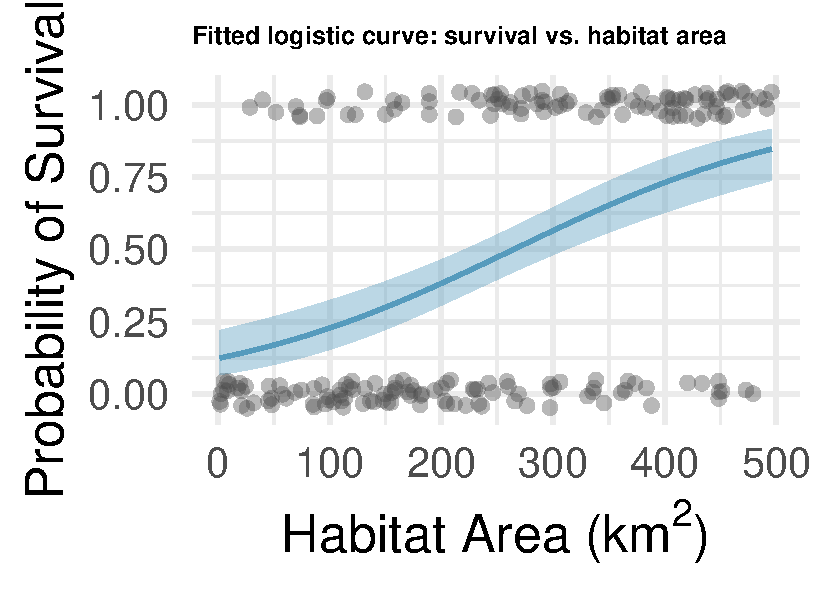
\includegraphics[width=0.66\textwidth]{survival_curve.pdf}
\end{center}

\pause
\vspace{-0.3em}
{\small One predictor at a time: survival probability climbs with habitat area, along a smooth S-shaped logistic curve, never leaving $[0,1]$ as a straight line would.}

\end{frame}


%%%%%%%%%%%%%%%%%%%%%%%%%%%%%%%%%%%%%%%%%%%%%%%%%%%%%%%%%%%%%%%%%%%%%%%%
\section{Conditions for valid inference}
%%%%%%%%%%%%%%%%%%%%%%%%%%%%%%%%%%%%%%%%%%%%%%%%%%%%%%%%%%%%%%%%%%%%%%%%
\begin{frame}
\frametitle{What the tests and intervals rely on}

For the tests and CIs to be trustworthy:

\pause
\vspace{0.2em}
{\small
\begin{enumerate}\setlength{\itemsep}{2pt}
\item \textbf{Independence:} each species independent of the others.
\item \textbf{Linearity in the log-odds:} linear in each predictor (\emph{not} the probability, which is S-shaped).
\item \textbf{Enough data:} roughly $\geq 10$ events \emph{and} $\geq 10$ non-events per predictor.
\end{enumerate}}

\pause
\vspace{0.2em}
\caution{No normality, no equal variance. Those were about a continuous error term. Here the response is Bernoulli, its variance $p(1-p)$ fixed by the mean. The conditions change with the response.}

\end{frame}


%%%%%%%%%%%%%%%%%%%%%%%%%%%%%%%%%%%%%%%%%%%%%%%%%%%%%%%%%%%%%%%%%%%%%%%%
\begin{frame}
\frametitle{Checking linearity in the log-odds}

Bin a predictor, compute the empirical log-odds $\log\frac{\hat p}{1-\hat p}$ in each bin, and plot against the predictor.

\pause
\vspace{0.2em}
\begin{center}
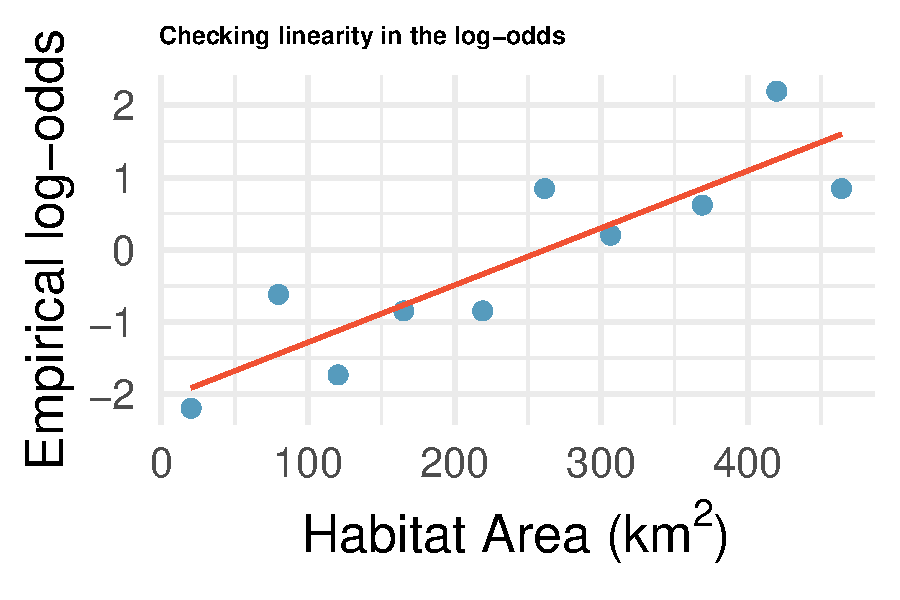
\includegraphics[width=0.58\textwidth]{logodds_linearity.pdf}
\end{center}

\pause
\vspace{-0.3em}
{\small Here the points track a line, so the log-odds linearity condition holds for \texttt{habitat\_area}.}

\end{frame}


%%%%%%%%%%%%%%%%%%%%%%%%%%%%%%%%%%%%%%%%%%%%%%%%%%%%%%%%%%%%%%%%%%%%%%%%
\section{Inference for a coefficient}
%%%%%%%%%%%%%%%%%%%%%%%%%%%%%%%%%%%%%%%%%%%%%%%%%%%%%%%%%%%%%%%%%%%%%%%%
\begin{frame}
\frametitle{One coefficient at a time}

Just like Lecture 14, one row of the table at a time, but the reference distribution is now a $z$ (normal), not a $t$.

\pause
\vspace{0.3em}
\formula{Test and interval for $\beta_j$}{To test $H_0: \beta_j = 0$, $$z = \frac{\hat\beta_j}{\mathrm{SE}(\hat\beta_j)} \;\overset{H_0}{\approx}\; N(0,1), \qquad p = 2\,P(Z > |z|).$$ A $95\%$ CI is $\hat\beta_j \pm z^\ast\,\mathrm{SE}(\hat\beta_j)$ with $z^\ast = 1.96$.}

\pause
\vspace{0.3em}
{\small The normal (not $t$) because logistic regression is fit by maximum likelihood, and MLE standard errors are \hl{asymptotic}: exact only as $n \to \infty$. Another reason the sample-size condition matters.}

\end{frame}


%%%%%%%%%%%%%%%%%%%%%%%%%%%%%%%%%%%%%%%%%%%%%%%%%%%%%%%%%%%%%%%%%%%%%%%%
\begin{frame}[fragile]
\frametitle{Reading the software output}

\begin{Verbatim}[fontsize=\small]
model <- glm(survived ~ habitat_area + population_size +
                        genetic_diversity + human_impact,
             family = binomial, data = species)
model |> tidy()
\end{Verbatim}

\pause
\vspace{0.2em}
\begin{Verbatim}[fontsize=\small]
  term               estimate std.error statistic  p.value
  (Intercept)        -2.00     0.641      -3.11    1.9e-3
  habitat_area        0.0112   0.00177     6.31    2.8e-10
  population_size     0.000421 0.000133    3.17    1.6e-3
  genetic_diversity   2.65     0.856       3.09    2.0e-3
  human_impact       -0.523    0.0839     -6.23    4.6e-10
\end{Verbatim}

\pause
\vspace{0.2em}
{\small Every predictor clears $p < 0.01$. The \texttt{statistic} column is the $z$, and the signs read directly: more habitat and diversity help; more human impact hurts.}

\end{frame}


%%%%%%%%%%%%%%%%%%%%%%%%%%%%%%%%%%%%%%%%%%%%%%%%%%%%%%%%%%%%%%%%%%%%%%%%
\begin{frame}
\frametitle{From a coefficient to an odds ratio}

The coefficient lives on the log-odds scale. \hl{Exponentiate} to get the odds ratio, and exponentiate the interval's endpoints for its CI:
$$\mathrm{OR} = e^{\hat\beta_j}, \qquad \left(e^{\hat\beta_j - z^\ast\mathrm{SE}},\; e^{\hat\beta_j + z^\ast\mathrm{SE}}\right).$$

\pause
\vspace{0.3em}
\textbf{\texttt{habitat\_area}:} $e^{0.0112} = 1.011$, 95\% CI $(1.008,\ 1.015)$.

{\small Each extra km$^2$ multiplies the odds of survival by $1.011$, tiny per km$^2$.}

\pause
\vspace{0.3em}
\keyidea{Scale the predictor to a meaningful step before interpreting. A \hl{$100$ km$^2$} increase multiplies the odds by $1.011^{100} = \hl{3.05}$, 95\% CI $(2.16,\ 4.31)$, so the odds of survival roughly \emph{triple}.}

\end{frame}


%%%%%%%%%%%%%%%%%%%%%%%%%%%%%%%%%%%%%%%%%%%%%%%%%%%%%%%%%%%%%%%%%%%%%%%%
\begin{frame}[fragile]
\frametitle{Odds ratios straight from R}

\begin{Verbatim}[fontsize=\small]
model |> tidy(conf.int = TRUE, exponentiate = TRUE) |>
  select(term, estimate, conf.low, conf.high)
\end{Verbatim}

\pause
\vspace{0.2em}
\begin{Verbatim}[fontsize=\small]
  term               estimate  conf.low  conf.high
  (Intercept)          0.136    0.0365     0.458
  habitat_area         1.011    1.008      1.015
  population_size      1.000    1.000      1.001
  genetic_diversity   14.09     2.758     80.55
  human_impact         0.593    0.497      0.691
\end{Verbatim}

\pause
\vspace{0.2em}
{\small An OR above $1$ raises the odds, below $1$ lowers them, and a CI straddling $1$ means ``no evidence of an effect.'' \texttt{genetic\_diversity} is dramatic, but its predictor only spans $0.1$ to $0.9$, so the honest step is a $0.1$ change, not a full unit.}

\end{frame}


%%%%%%%%%%%%%%%%%%%%%%%%%%%%%%%%%%%%%%%%%%%%%%%%%%%%%%%%%%%%%%%%%%%%%%%%
\section{Predicting a probability}
%%%%%%%%%%%%%%%%%%%%%%%%%%%%%%%%%%%%%%%%%%%%%%%%%%%%%%%%%%%%%%%%%%%%%%%%
\begin{frame}
\frametitle{A confidence interval for $p^\ast$}

For a new species $x^\ast$ we want a CI for $p^\ast = P(Y=1 \mid x^\ast)$. Build it \hl{on the log-odds scale, then transform}, the move from Lecture 15.

\pause
\vspace{0.2em}
{\small
\begin{enumerate}\setlength{\itemsep}{1pt}
\item Predict the log-odds $\hat\eta^\ast$ and $\mathrm{SE}(\hat\eta^\ast)$ (\texttt{predict(type="link")}).
\item CI on the log-odds scale: $\hat\eta^\ast \pm z^\ast\,\mathrm{SE}(\hat\eta^\ast)$.
\item Inverse-logit both endpoints: $p = 1/(1 + e^{-\eta})$.
\end{enumerate}}

\pause
\vspace{0.2em}
\keyidea{Transforming the \emph{endpoints} keeps the interval inside $[0,1]$. For a median species: log-odds $-0.51 \pm 0.43 \Rightarrow \hat p = 0.38$, 95\% CI $(0.28,\ 0.48)$. Never build the CI on the probability scale directly.}

\end{frame}


%%%%%%%%%%%%%%%%%%%%%%%%%%%%%%%%%%%%%%%%%%%%%%%%%%%%%%%%%%%%%%%%%%%%%%%%
\section{Diagnostics}
%%%%%%%%%%%%%%%%%%%%%%%%%%%%%%%%%%%%%%%%%%%%%%%%%%%%%%%%%%%%%%%%%%%%%%%%
\begin{frame}
\frametitle{Do the predictions separate the outcomes?}

\begin{center}
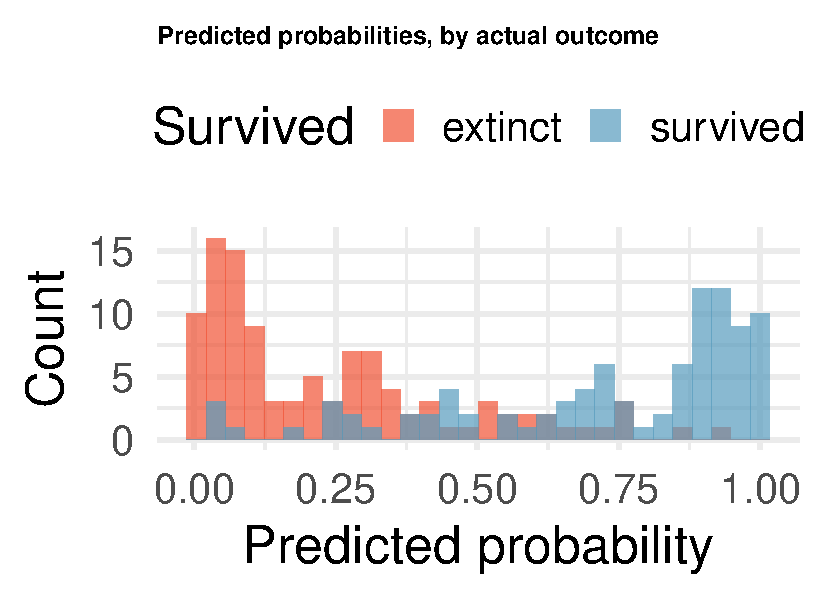
\includegraphics[width=0.62\textwidth]{predicted_probs.pdf}
\end{center}

\pause
\vspace{-0.3em}
{\small Colored by the actual outcome. A good model pushes survivors right and extinctions left; overlap in the middle is where it is unsure, and some overlap is honest.}

\end{frame}


%%%%%%%%%%%%%%%%%%%%%%%%%%%%%%%%%%%%%%%%%%%%%%%%%%%%%%%%%%%%%%%%%%%%%%%%
\begin{frame}
\frametitle{Binned residuals}

Individual $0/1$ residuals are useless to eyeball, so \hl{bin} by fitted probability and average the residual in each bin.

\pause
\begin{center}
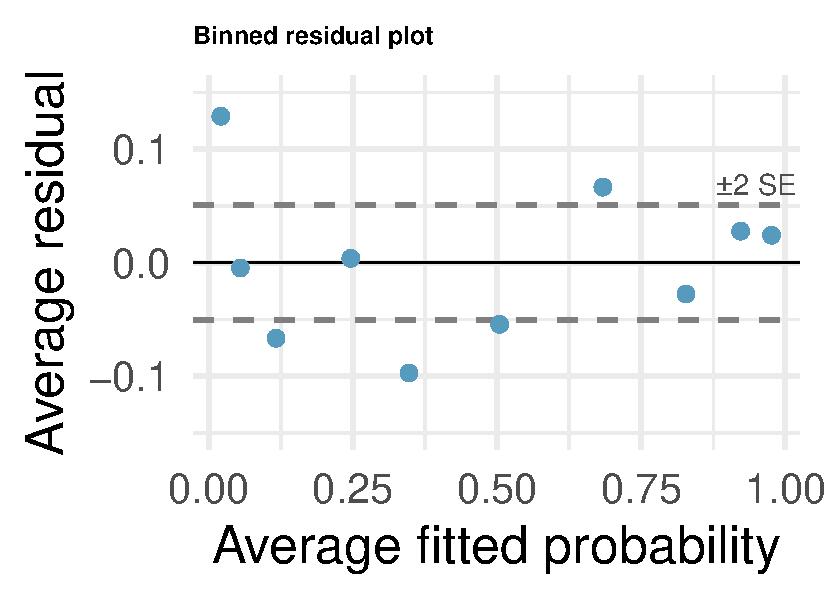
\includegraphics[width=0.52\textwidth]{binned_residuals.pdf}
\end{center}

\pause
\vspace{-0.4em}
{\small Bin averages should scatter around $0$ inside the $\pm 2\,\mathrm{SE}$ band. Strays signal a missing term or the wrong form.}

\end{frame}


%%%%%%%%%%%%%%%%%%%%%%%%%%%%%%%%%%%%%%%%%%%%%%%%%%%%%%%%%%%%%%%%%%%%%%%%
\section{Prediction and cross-validation}
%%%%%%%%%%%%%%%%%%%%%%%%%%%%%%%%%%%%%%%%%%%%%%%%%%%%%%%%%%%%%%%%%%%%%%%%
\begin{frame}
\frametitle{From a probability to a decision}

The model outputs a \emph{probability} $\hat p_i$. To make a call, pick a threshold $c$ (often $0.5$): predict $\hat Y_i = 1$ if $\hat p_i \geq c$.

\pause
\vspace{0.3em}
Comparing $\hat Y_i$ to the truth gives the \hl{confusion matrix}:

\vspace{0.2em}
\begin{center}
\begin{tabular}{lcc}
\toprule
& \textbf{Predicted 1} & \textbf{Predicted 0} \\
\midrule
\textbf{Actual 1} & True Positive & False Negative \\
\textbf{Actual 0} & False Positive & True Negative \\
\bottomrule
\end{tabular}
\end{center}

\pause
\vspace{0.3em}
{\small The \hl{misclassification rate} is $(\mathrm{FP} + \mathrm{FN})/n$, the fraction the model got wrong.}

\end{frame}


%%%%%%%%%%%%%%%%%%%%%%%%%%%%%%%%%%%%%%%%%%%%%%%%%%%%%%%%%%%%%%%%%%%%%%%%
\begin{frame}
\frametitle{Accuracy can lie}

\caution{With \hl{imbalanced} outcomes, accuracy is a trap. If $90\%$ of species survived, ``predict survived for everyone'' scores $90\%$ accuracy while missing \emph{every single} extinction. The threshold $c = 0.5$ is a default, not a law.}

\pause
\vspace{0.4em}
Two ways out:
\begin{itemize}
\item move the threshold to match the \emph{costs} of the two errors;
\pause
\item score the \hl{probabilities} directly, and never pick a threshold at all.
\end{itemize}

\end{frame}


%%%%%%%%%%%%%%%%%%%%%%%%%%%%%%%%%%%%%%%%%%%%%%%%%%%%%%%%%%%%%%%%%%%%%%%%
\begin{frame}
\frametitle{Two losses for probabilities}

For a continuous $Y$ we scored predictions with squared error. For a probability, two standard replacements:

\pause
\vspace{0.3em}
\formula{Brier score and log-loss}{\vspace{-0.7em}\begin{align*} \text{Brier} &= \tfrac{1}{n}\textstyle\sum_{i=1}^n (y_i - \hat p_i)^2 \\[0.2em] \text{Log-loss} &= -\tfrac{1}{n}\textstyle\sum_{i=1}^n \big[y_i \log \hat p_i + (1-y_i)\log(1-\hat p_i)\big] \end{align*}\vspace{-0.7em}\\ Brier is MSE on probabilities (range $[0,1]$); log-loss is the negative average log-likelihood (range $[0,\infty)$). Lower is better.}

\pause
\vspace{0.3em}
{\small Both are $0$ for a perfect confident call. To see how they \emph{differ}, look at one observation at a time.}

\end{frame}


%%%%%%%%%%%%%%%%%%%%%%%%%%%%%%%%%%%%%%%%%%%%%%%%%%%%%%%%%%%%%%%%%%%%%%%%
\begin{frame}
\frametitle{Per-observation loss}

\textbf{The loss when the truth is $y_i = 1$}, as the predicted $\hat p_i$ moves from confident-right to confident-wrong:

\vspace{0.4em}
\begin{center}
\begin{tabular}{lccccc}
\toprule
$\hat p_i$ & $0.99$ & $0.80$ & $0.50$ & $0.20$ & $0.01$ \\
\midrule
Brier $(y_i-\hat p_i)^2$ & $0.00$ & $0.04$ & $0.25$ & $0.64$ & $0.98$ \\
Log-loss $-\log \hat p_i$   & $0.01$ & $0.22$ & $0.69$ & $1.61$ & $\hl{4.61}$ \\
\bottomrule
\end{tabular}
\end{center}

\pause
\vspace{0.4em}
{\small Both climb as the prediction gets worse. But at the confident-wrong end ($\hat p = 0.01$) Brier is capped near $1$ while log-loss shoots to $\hl{4.61}$, heading to $\infty$ as $\hat p \to 0$.}

\end{frame}


%%%%%%%%%%%%%%%%%%%%%%%%%%%%%%%%%%%%%%%%%%%%%%%%%%%%%%%%%%%%%%%%%%%%%%%%
\begin{frame}
\frametitle{Brier vs.\ log-loss: the difference}

\dq{Both are $0$ for a perfect confident call. So when does it matter which you use?}

\pause
\vspace{0.4em}
\keyidea{When the model is \hl{confidently wrong}. Predicting $\hat p = 0.01$ for a species that \emph{did} survive costs Brier $0.98$ but log-loss $\mathbf{4.61}$. Log-loss punishes overconfident mistakes far more harshly. Use it when a sure-but-wrong prediction is the expensive kind of error.}

\pause
\vspace{0.3em}
{\small And both \hl{sidestep the threshold} entirely: they grade the probabilities themselves, so there is no $c$ to choose.}

\end{frame}


%%%%%%%%%%%%%%%%%%%%%%%%%%%%%%%%%%%%%%%%%%%%%%%%%%%%%%%%%%%%%%%%%%%%%%%%
\begin{frame}
\frametitle{Choosing the threshold}

\dq{Should we always use $c = 0.5$?}

\pause
\vspace{0.3em}
It depends on which error costs more:
\begin{itemize}
\item \textbf{Conservation triage:} missing an at-risk species (FN) is worse than a false alarm (FP). Lower the threshold ($c = 0.3$) to flag more species.
\pause
\item \textbf{Spam filter:} blocking a real email (FP) is worse than a stray spam (FN). Raise it ($c = 0.9$).
\end{itemize}

\pause
\vspace{0.3em}
{\small The threshold is a \emph{decision}, not a statistic. It belongs to whoever pays for the mistakes.}

\end{frame}


%%%%%%%%%%%%%%%%%%%%%%%%%%%%%%%%%%%%%%%%%%%%%%%%%%%%%%%%%%%%%%%%%%%%%%%%
\begin{frame}
\frametitle{Cross-validation, now for classification}

The Lecture 15 machinery, unchanged, with only the loss swapped.

\pause
\vspace{0.3em}
\formula{$k$-fold CV for logistic regression}{%
\begin{enumerate}\setlength{\itemsep}{1pt}
\item Pick a loss: misclassification, Brier, or log-loss.
\item Split into $k$ folds. For each fold $j$, fit on the other $k-1$, predict $\hat p_i$ on fold $j$, average the loss over it.
\end{enumerate}
$$\text{CV-error} = \frac{1}{k}\sum_{j=1}^{k}\mathrm{err}_j.$$}

\pause
\vspace{0.3em}
{\small Same benefits as before: few assumptions, and you \hl{choose the loss to match the analysis}. On the species data ($5$-fold, $20$ repeats) the full model beats a two-predictor one on all three losses: misclassification $0.19$ vs $0.30$, log-loss $0.44$ vs $0.59$.}

\end{frame}


%%%%%%%%%%%%%%%%%%%%%%%%%%%%%%%%%%%%%%%%%%%%%%%%%%%%%%%%%%%%%%%%%%%%%%%%
\section{Wrap-up}
%%%%%%%%%%%%%%%%%%%%%%%%%%%%%%%%%%%%%%%%%%%%%%%%%%%%%%%%%%%%%%%%%%%%%%%%
\begin{frame}
\frametitle{Linear vs.\ logistic inference, side by side}

{\small
\begin{center}
\renewcommand{\arraystretch}{1.25}
\begin{tabular}{lll}
\toprule
& \textbf{Linear regression} & \textbf{Logistic regression} \\
\midrule
Response & continuous $Y$ & binary $Y \in \{0,1\}$ \\
Model & $Y = \beta_0 + \beta_1 X + \varepsilon$ & $\log\frac{p}{1-p} = \beta_0 + \beta_1 X$ \\
Fit by & least squares & maximum likelihood \\
\midrule
Statistic & $t = \hat\beta / \mathrm{SE}$ & $z = \hat\beta / \mathrm{SE}$ \\
Null dist. & $t_{n-p-1}$ (exact) & $N(0,1)$ (asymptotic) \\
CI for $\beta$ & $\hat\beta \pm t^\ast\,\mathrm{SE}$ & $\hat\beta \pm z^\ast\,\mathrm{SE}$ \\
\midrule
$\hat\beta$ means & $\hat\beta$ units of $Y$ per unit $X$ & odds $\times\, e^{\hat\beta}$ per unit $X$ \\
Conditions & LINE & independence, log-odds \\
& & linearity, large $n$ \\
\bottomrule
\end{tabular}
\end{center}}

\end{frame}


%%%%%%%%%%%%%%%%%%%%%%%%%%%%%%%%%%%%%%%%%%%%%%%%%%%%%%%%%%%%%%%%%%%%%%%%
\begin{frame}
\frametitle{Summary}

\begin{itemize}
\item Logistic regression models the \hl{log-odds} linearly; $e^{\hat\beta_j}$ is an \hl{odds ratio}. Fit by maximum likelihood.
\item Test a coefficient with $z = \hat\beta_j/\mathrm{SE} \sim N(0,1)$; interval $\hat\beta_j \pm z^\ast\mathrm{SE}$. \hl{Exponentiate} the endpoints for the odds-ratio CI, and scale the predictor to a meaningful step.
\item For a predicted probability, build the CI on the log-odds scale and \hl{inverse-logit the endpoints}, so it stays in $[0,1]$.
\item Conditions: independence, \hl{linearity in the log-odds}, a large enough sample. Check with the log-odds and binned-residual plots.
\item Score probabilities with the \hl{Brier score} or \hl{log-loss}, and log-loss punishes confident mistakes hardest. Select models by cross-validation, with the loss of your choosing.
\end{itemize}

\end{frame}


%%%%%%%%%%%%%%%%%%%%%%%%%%%%%%%%%%%%%%%%%%%%%%%%%%%%%%%%%%%%%%%%%%%%%%%%
\begin{frame}
\frametitle{Coming up next}

\hl{That closes Module 3.} Five lectures on regression inference: the slope, multiple regression, transformations and interactions, prediction and cross-validation, and now logistic.

\vspace{0.4em}
\begin{itemize}
\item \hl{Lecture 17 is next, a whole new module.} Everything so far has been frequentist: the parameter is fixed, the interval is random.
\item \hl{Bayesian statistics} turns that around: the parameter gets a distribution, and ``$95\%$'' will mean something different. It opens with priors, updating, and how belief becomes a posterior (Bayes Rules!\ Chs.\ 1, 2, and 4).
\item The \hl{linear-vs-logistic table} is your one-page summary of Module 3.
\end{itemize}

\end{frame}


%%%%%%%%%%%%%%%%%%%%%%%%%%%%%%%%%%%%%%%%%%%%%%%%%%%%%%%%%%%%%%%%%%%%%%%%
% Activity
%%%%%%%%%%%%%%%%%%%%%%%%%%%%%%%%%%%%%%%%%%%%%%%%%%%%%%%%%%%%%%%%%%%%%%%%
\begin{frame}
\frametitle{Activity: what raises the risk of heart disease?}

\activity{$208$ Cleveland heart-disease patients, labeled with heart disease or not. Fit a logistic model from age, blood pressure, cholesterol and max heart rate, then
\begin{itemize}\setlength{\itemsep}{1pt}
\item read each coefficient as an odds ratio with its CI;
\item check the conditions;
\item compare models by cross-validation, with a loss that fits a medical screen.
\end{itemize}}

\vspace{0.3em}
{\small
\begin{itemize}
\item Work in \emph{pairs} (analyst + guide), one worksheet per pair.
\item We pause for check-ins. \hl{Be ready to share}.
\item Data and starter code are on Blackboard.
\end{itemize}}

\end{frame}


%%%%%%%%%%%%%%%%%%%%%%%%%%%%%%%%%%%%%%%%%%%%%%%%%%%%%%%%%%%%%%%%%%%%%%%%
\begin{frame}
\frametitle{Compare with the groups around you}

\textbf{When you reach the end of Part 5:}

\vspace{0.3em}
\begin{enumerate}
\item Compare your final model with at least two neighboring pairs.
\item Did everyone read the cholesterol odds ratio the same way: per unit, or per meaningful step?
\item For a screening test, would you set the threshold above or below $0.5$? Did your neighbors agree?
\item Having heard them, would you change your model or your threshold?
\end{enumerate}

\vspace{0.5em}
\hl{Write your answers in the box at the end of the worksheet.}

\end{frame}


%%%%%%%%%%%%%%%%%%%%%%%%%%%%%%%%%%%%%%%%%%%%%%%%%%%%%%%%%%%%%%%%%%%%%%%%
% End document
%%%%%%%%%%%%%%%%%%%%%%%%%%%%%%%%%%%%%%%%%%%%%%%%%%%%%%%%%%%%%%%%%%%%%%%%

\end{document}
